\chapter{Qnorm: fast-ish (and correct!) quantile normalization in Python}\thumbforchapter
\chaptermark{Qnorm}
\chapterauthor{Maarten van der Sande, Simon J. van Heeringen}
\newpage
\definecolor{bash_backcolor}{RGB}{48,10,36}

Quantile normalization made easy! This tool was developed as the current (Python) implementations scattered across the web do not correctly resolve collisions/ties in the ranks. Properly resolving rank ties is important when ties happen frequently, such as when working with discrete numbers (integers) in count tables. This implementation should be relatively fast, and can use multiple cores to sort the columns and tie-resolvement is accelerated by numba.

\section{Code example}

We recreate the example of Wikipedia\footnote{\url{https://en.wikipedia.org/wiki/Quantile_normalization}}:

\begin{lstlisting}[language=Python]
import pandas as pd
import qnorm

df = pd.DataFrame({'C1': {'A': 5, 'B': 2, 'C': 3, 'D': 4},
                   'C2': {'A': 4, 'B': 1, 'C': 4, 'D': 2},
                   'C3': {'A': 3, 'B': 4, 'C': 6, 'D': 8}})

print(qnorm.quantile_normalize(df, axis=1))

         C1        C2        C3
A  5.666667  5.166667  2.000000
B  2.000000  2.000000  3.000000
C  3.000000  5.166667  4.666667
D  4.666667  3.000000  5.666667
\end{lstlisting}

It is important to note that qnorm standardizes along columns by default, like in the wiki example above. However \lstinline[language=Python]{qnorm.quantile_normalize} accepts an (optional) axis argument, which can be used to change this behaviour. If \lstinline[language=Python]{axis=1} (default), standardize along columns, if \lstinline[language=Python]{axis=0`}, standardize along rows.

\begin{itemize}
    \item note: pandas is an optional dependency of qnorm, and if you want to quantile normalize dataframes make sure to install pandas yourself (conda/pip install pandas).

    \item note: you can also pass numpy arrays as input to \lstinline[language=Python]{qnorm.quantile_normalize}.
\end{itemize}

\section{Multicore support}

To accelerate the computation you can pass a ncpus argument to the function call and qnorm will be run in parallel:

\begin{lstlisting}[language=Python]
qnorm.quantile_normalize(df, ncpus=8)  
\end{lstlisting}

\section{Normalize onto distribution}

You can also use the \lstinline[language=Python]{qnorm.quantile_normalize} function to normalize "onto" a distribution, by passing a target along to the function call.

\begin{lstlisting}[language=Python]
import pandas as pd
import qnorm

df = pd.DataFrame({'C1': {'A': 4, 'B': 3, 'C': 2, 'D': 1},
                   'C2': {'A': 1, 'B': 2, 'C': 3, 'D': 4}})

print(qnorm.quantile_normalize(df, target=[8, 9, 10, 11]))

     C1    C2
A  11.0   8.0
B  10.0   9.0
C   9.0  10.0
D   8.0  11.0
\end{lstlisting}

\section{How fast is it and what is its memory usage?}

How better to measure this than a little benchmark/example? For this example, we will consider 100 replicates, each consisting of one million integer values between 0 and 100, which should give us plenty of rank ties.

\begin{lstlisting}[language=Python]
import numpy as np
import qnorm

test = np.random.randint(0, 100, size=(1_000_000, 100), dtype=np.int32)

qnorm.quantile_normalize(test, ncpus=4)
\end{lstlisting}

Of which we can now check how long it takes with a little bash script:

\begin{mdframed}[
    backgroundcolor=bash_backcolor,
    hidealllines=true,
    innertopmargin=0pt,
    innerbottommargin=0pt,
    innerleftmargin=0pt,
    innerrightmargin=0pt
]
\begin{lstlisting}[escapechar=\%,language=bash,basicstyle=\ttfamily\color{white}]
user@comp:%$\mathtt{\sim}$%$ /usr/bin/time --verbose python small_qnorm_script.py \
|& grep -P "(wall clock|Maximum resident set size)"

Elapsed (wall clock) time (h:mm:ss or m:ss): 0:07.52
Maximum resident set size (kbytes): 2768884
\end{lstlisting}
\end{mdframed}

It takes only 7.5 seconds to initialize our table and quantile normalize it. I think that's pretty fast!

The test array we made consists of 100 * 1.000.000 = 100.000.000 single point precision integers, so four bytes each (400.000.000 bytes, 0.4 gigabytes). The memory footprint of our script is 0.27 gigabytes, around 7 times our input. Unfortunately that makes qnorm a bit memory hungry, but that should not be a problem in 99\% of the cases. If memory usage is a problem take a look at the supported low-memory implementation.

\subsection{Scaling of ncpus}

Using more than four cpus generally does not lead to a much bigger speedup.

\begin{figure}[H]
	\centering
	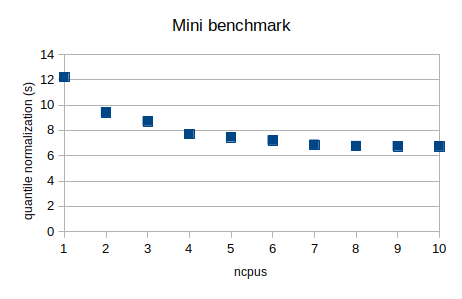
\includegraphics[width=0.5\textwidth]{ch.qnorm/imgs/benchmark_cores.png}
	\caption{\label{fig:benchmark_cores}\textbf{Qnorm wall clock time for different number of cores.}}
\end{figure}

\subsection{Incremental quantile norm}

In case you want to quantile normalize excessively large tables, there is a ``memory-efficient'' implementation. This implementation gets its memory efficiency by calculating the mean ``online'', which means we calculate it on fractions of the total table and then update the value. The other change is that intermediate results are written to disk. This means that this implementation effectively swaps memory to disk, and thus is not ``memory hungry'', but instead ``disk hungry''. This incremental method however can scale to virtually infinitely large tables (or until you run out of disk space).

Let's say we want to do something crazy like quantile normalize the human genome in 10 basepair bins. That means we will have around 300.000.000 values per sample. File-based qnorm works with both csv/tsv, parquet, and hdf files. For this example, we will work with hdf files (make sure to set \lstinline[language=Python]{data_columns=True}). Parquet and hdf files also are fast, but csv/tsv files are (very) slow because of the enormous amount of I/O they require.

\begin{lstlisting}[language=Python]
df = pd.DataFrame(
    index=range(300_000_000), 
    dtype=int, 
    columns=['sample'+str(col) for col in range(64)]
)
df[:] = np.random.randint(0, 100, size=df.shape)
df.to_hdf('hg_bins.hdf', key='qnorm', format='table', data_columns=True)
\end{lstlisting}

We can now compare the speed and memory of the file-based method vs the "standard" method.

\begin{lstlisting}[language=Python]
import qnorm

# incremental qnorm (reads hg_bins.hdf from disk and writes
# output to hg_bins_qnorm.hdf) 
qnorm.incremental_quantile_normalize(
    'hg_bins.hdf', 
    'hg_bins_qnorm.hdf', 
    rowchunksize=500_000, 
    colchunksize=4, 
    ncpus=4
)

# standard
df = pd.read_hdf(f'hg_bins.hdf').astype('float32')
df_qnorm = qnorm.quantile_normalize(df, ncpus=4)
\end{lstlisting}

\begin{figure}[H]
	\centering
	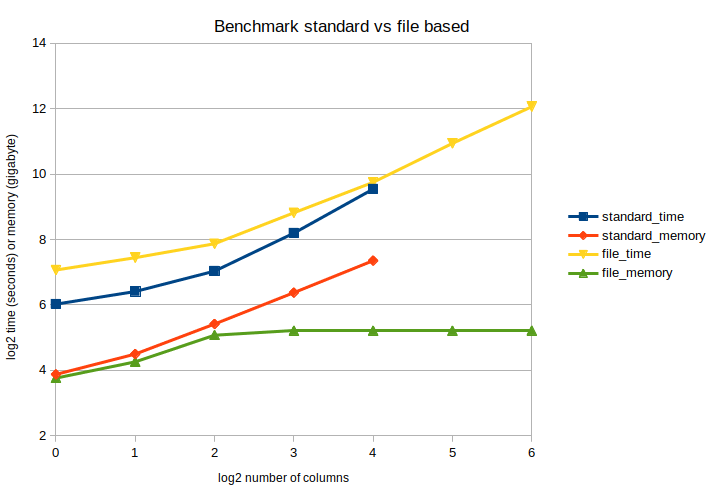
\includegraphics[width=0.5\textwidth]{ch.qnorm/imgs/benchmark_file.png}
	\caption{\label{fig:benchmark_file}\textbf{Qnorm wall clock time and memory usage for standard and file-based quantile normalization.} The benchmark was run on a dataset with 300.000.000 rows.}
\end{figure}

The standard method does not come farther than $2^4=16$ samples before running out of memory on a 512-gigabyte system! The incremental method has similar timings and even seems to scale better than the standard method for large arrays. And it takes only an hour to normalize 64 samples.

The rowchunksize and colchunksize respectively influence how large of chunks the output is written to disk and how many columns are being sorted and quantile normalized at the same time. Generally speaking, the larger the better, however, the defaults should most of the time be sufficiently fast.

\begin{itemize}
    \item note: Both in-memory normalization and incremental normalization should produce identical results, and neither is more correct than the other.

    \item note: note: The incremental implementation requires pandas to be installed (conda/pip install pandas).

    \item note: When using hdf files make sure to install (py)tables (conda install pytables or pip install tables).

    \item note: When using parquet files make sure to install pyarrow (conda install pyarrow or pip install pyarrow).

    \item note: The input format specifies the output format.

    \item note: Because of the design of hdf5, there is a limit on the number of columns it can hold. In case you have a lot of columns (500+), it is probably best to use parquet and not hdf5.

\end{itemize}

\section{Command Line Interface (CLI) example}

Qnorm also contains a CLI for converting csv/tsv files. The CLI depends on pandas, but this is an optional dependency of qnorm. To make use of the CLI make sure to install pandas in your current environment as well!

\begin{mdframed}[
    backgroundcolor=bash_backcolor,
    hidealllines=true,
    innertopmargin=0pt,
    innerbottommargin=0pt,
    innerleftmargin=0pt,
    innerrightmargin=0pt
]
\begin{lstlisting}[escapechar=\%,language=bash,basicstyle=\ttfamily\linespread{1.15}\footnotesize\color{white}]
user@comp:%$\mathtt{\sim}$%$ qnorm --help

usage: qnorm [-h] [-v] table

Quantile normalize your table

positional arguments:
  table          input csv/tsv file which will be quantile normalized

optional arguments:
  -h, --help     show this help message and exit
  -v, --version  show program's version number and exit
\end{lstlisting}
\end{mdframed}

And again the example of Wikipedia:

\begin{mdframed}[
    backgroundcolor=bash_backcolor,
    hidealllines=true,
    innertopmargin=0pt,
    innerbottommargin=0pt,
    innerleftmargin=0pt,
    innerrightmargin=0pt
]
\begin{lstlisting}[escapechar=\%,language=bash,basicstyle=\ttfamily\linespread{1.15}\footnotesize\color{white}]
user@comp:%$\mathtt{\sim}$%$ cat table.tsv
        C1      C2      C3
A       5       4       3
B       2       1       4
C       3       4       6
D       4       2       8

user@comp:%$\mathtt{\sim}$%$ qnorm table.tsv
        C1                C2                C3
A       5.66666666666     5.16666666666     2.0
B       2.0               2.0               3.0
C       3.0               5.16666666666     4.66666666666
D       4.66666666666     3.0               5.66666666666
\end{lstlisting}
\end{mdframed}

\begin{itemize}
    \item note: the qnorm cli assumes that the first column and the first row are used as descriptors, and are "ignored" in the quantile normalization process. Lines starting with a hashtag "\#" are treated as comments and ignored.

    \item note: The CLI requires pandas to be installed (conda/pip install pandas)
\end{itemize}

\section{Installation}

\subsection{pip}

\begin{lstlisting}[escapechar=\%,language=bash,basicstyle=\ttfamily\color{white}]
user@comp:%$\mathtt{\sim}$%$ pip install qnorm
\end{lstlisting}

\subsection{conda}

Installing qnorm from the conda-forge channel can be achieved by adding conda-forge to your channels with:

\begin{lstlisting}[escapechar=\%,language=bash,basicstyle=\ttfamily\color{white}]
user@comp:%$\mathtt{\sim}$%$ conda config --add channels conda-forge
\end{lstlisting}

Once the conda-forge channel has been enabled, qnorm can be installed with:

\begin{lstlisting}[escapechar=\%,language=bash,basicstyle=\ttfamily\color{white}]
user@comp:%$\mathtt{\sim}$%$ conda install qnorm
\end{lstlisting}

\subsection{local}

clone the repository

\begin{lstlisting}[escapechar=\%,language=bash,basicstyle=\ttfamily\color{white}]
user@comp:%$\mathtt{\sim}$%$ git clone https://github.com/Maarten-vd-Sande/qnorm
\end{lstlisting}

And install it

\begin{mdframed}[
    backgroundcolor=bash_backcolor,
    hidealllines=true,
    innertopmargin=0pt,
    innerbottommargin=0pt,
    innerleftmargin=0pt,
    innerrightmargin=0pt
]
\begin{lstlisting}[language=bash,basicstyle=\ttfamily\color{white}]
user@comp:%$\mathtt{\sim}$%$ cd qnorm
user@comp:%$\mathtt{\sim}$%$ pip install .
\end{lstlisting}
\end{mdframed}
